\section{Experiments}

\subsection{Reproducing the results of \textcite{frenayParameterinsensitiveKernelExtreme2011}}
\label{sec:reproducing-frenay}

% \begin{figure}[H]
% 	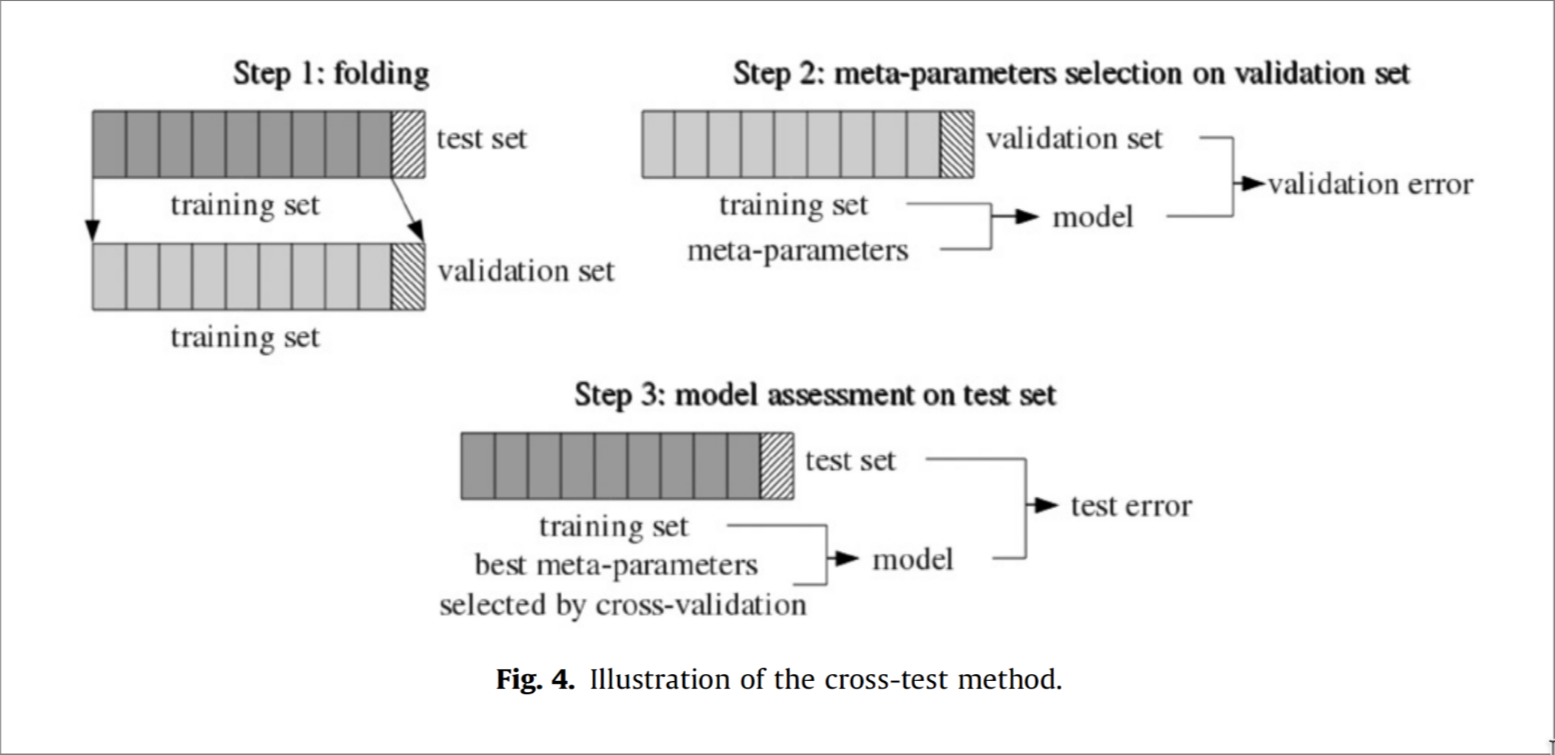
\includegraphics{frenay-cross-test}
% 	\caption{Illustration of the cross-test method from \cite{frenayParameterinsensitiveKernelExtreme2011}}
% 	\label{fig:frenay-cross-test}
% \end{figure}

In the paper, \textcite{frenayParameterinsensitiveKernelExtreme2011} use a double cross-test resampling
method which is illustrated in \cref{fig:frenay-cross-test}. First, they perform a 10-fold cross validation,
where the 9 folds of the training set are then used on a second 10-fold cross validation to determine the
best hyperparameters. This means that there are 100 training processes in total.

\begin{figure}[H]
    \begin{tikzpicture}[
		scale=0.66,
		every node/.style={font=\footnotesize},
	]
	% Draw main rectangle
	\def\nfolds{10}
	\pgfmathsetmacro{\trainfolds}{\nfolds-1}
	\pgfmathsetmacro{\splits}{\nfolds-2}
	\def\heightmult{0.5}

	\newcommand{\fold}[5]{%
		\draw[#2] #1 rectangle ($#1+(\heightmult*\trainfolds,1)$);
		% fill with pattern
		\filldraw[#3] ($#1+(\heightmult*\trainfolds,0)$) rectangle ($#1+(\heightmult*\nfolds,1)$);

		\draw ($#1+(\heightmult*\trainfolds/2,0)$) node[below,name=below-#5] {training set};
		\draw ($#1+(\heightmult*\nfolds,0.5)$) node[right,name=right-#5] {#4 set};

		% Draw vertical dashed lines for fold divisions
		\foreach \x in {1,...,\splits}{
				\draw ($#1+(\heightmult*\x,0)$) -- ($#1+({\heightmult*\x},1)$);
			}
	}

	\def\coltest{wong_blue}
	\def\colvali{wong_orange}

	\fill[shading=axis,top color=\coltest!40,bottom color=\colvali!40] (0,0) -- (\heightmult*\trainfolds,0) -- (\heightmult*\nfolds,-1) -- (0,-1) -- cycle;

	\fold{(0,0)}{fill=\coltest}{pattern=north east lines, pattern color=\coltest}{test}{test1}
	\fold{(0,-2)}{fill=\colvali}{pattern=north west lines,pattern color=\colvali}{validation}{val1}

	\draw[->] (0,0) -- (0,-1);
	\draw[->] (\heightmult*\trainfolds,0) -- (\heightmult*\nfolds,-1);

	% title above bounding box
	% \draw (current bounding box.north) node[above] {\textbf{Step 1: folding}};

	\fold{(9,0)}{fill=\colvali}{pattern=north west lines,pattern color=\colvali}{validation}{val2}

	\draw (right-val1.east -| below-val2.south) node[name=meta-parameters] {meta-parameters};
	\coordinate (a) at ($(meta-parameters)!.5!(below-val2)$);
	\node[name=model] at (a -| right-val2) {model};

	\coordinate (vm) at ($(model)!.5!(right-val2)$);
	\node[name=valerr] at ($(vm)+(5,0)$) {validation error};

	\coordinate (mm) at ($(meta-parameters.east |- model.west)!0.5!(model.west)$);
	\draw (below-val2.east) -| (mm);
	\draw (meta-parameters.east) -| (mm);
	\draw[->] (mm) -- (model);

	\coordinate (vvm) at ($(right-val2.east |- valerr.west)!0.5!(valerr.west)$);
	\draw (right-val2.east) -| (vvm);
	\draw (model.east) -| (vvm);
	\draw[->] (vvm) -- (valerr);

	% step 3

	\coordinate (step3) at (5,-5);
	\fold{(step3)}{fill=\coltest}{pattern=north east lines,pattern color=\coltest}{test}{test3}

	\draw ($(below-test3.south)+(0,-1)$) node[name=best-meta-parameters,text width=3cm,align=center]
	{best meta-parameters selected by cross-validation};

	\coordinate (b) at ($(best-meta-parameters)!.5!(below-test3)$);
	\node[name=model3] at ($(b -| right-test3)+(1,0)$) {model};

	\coordinate (vm3) at ($(model3)!.5!(right-test3)$);
	\node[name=testerr] at ($(vm3)+(5,0)$) {test error};

	\coordinate (mm3) at ($(best-meta-parameters.east |- model3.west)!0.5!(model3.west)$);
	\draw (below-test3.east) -| (mm3);
	\draw (best-meta-parameters.east) -| (mm3);
	\draw[->] (mm3) -- (model3);

	\coordinate (vvm3) at ($(right-test3.east |- testerr.west)!0.5!(testerr.west)$);
	\draw (right-test3.east) -| (vvm3);
	\draw (model3.east) -| (vvm3);
	\draw[->] (vvm3) -- (testerr);

	\coordinate (shift) at (0,1.5);
	\draw ($(0,0)+(shift)$) node[right] {\textbf{Step 1: folding}};
	\draw ($(9,0)+(shift)$) node[right] {\textbf{Step 2: meta-parameters selection on validation set}};
	\draw ($(step3)+(shift)$) node[right] {\textbf{Step 3: model assessment on test set}};

	% \draw ($(9,0)!0.5!(valerr.east) + (0,1.1)$) node[above] {\textbf{Step 2: meta-parameters selection on validation set}};

	% \draw ($(step3)!0.5!(step3 -| testerr.east) + (0,1)$) node[above] {\textbf{Step 3: model assessment on test set}};

\end{tikzpicture}

	\caption{Illustration of the cross-test method from \cite{frenayParameterinsensitiveKernelExtreme2011}}
	\label{fig:frenay-cross-test}
\end{figure}


\subsection{Comparing the performance of the kernels with different datasets}

\subsubsection{Resampling}

Instead of using the double cross-test resampling used in \cref{sec:reproducing-frenay},
we opted to use a 5-2 cross-validation resampling method as described by \textcite{dietterichApproximateStatisticalTests1998}.

The 5-2 cross-validation
consists of doing a 50-50 split of the dataset into two sets. First, we train on the first set and test on the second set
and then we train on the second set and test on the first set. The process is repeated 5 times, each time
with a different random split. We choose this method since it is faster then the double cross-test method
requiring only 10 training processes instead of 100.

% TODO: Add figure of the 5-2 cross-validation


\begin{figure}
    % Recommended preamble:
% \usetikzlibrary{arrows.meta}
% \usetikzlibrary{backgrounds}
% \usepgfplotslibrary{patchplots}
% \usepgfplotslibrary{fillbetween}
% \pgfplotsset{%
%     layers/standard/.define layer set={%
%         background,axis background,axis grid,axis ticks,axis lines,axis tick labels,pre main,main,axis descriptions,axis foreground%
%     }{
%         grid style={/pgfplots/on layer=axis grid},%
%         tick style={/pgfplots/on layer=axis ticks},%
%         axis line style={/pgfplots/on layer=axis lines},%
%         label style={/pgfplots/on layer=axis descriptions},%
%         legend style={/pgfplots/on layer=axis descriptions},%
%         title style={/pgfplots/on layer=axis descriptions},%
%         colorbar style={/pgfplots/on layer=axis descriptions},%
%         ticklabel style={/pgfplots/on layer=axis tick labels},%
%         axis background@ style={/pgfplots/on layer=axis background},%
%         3d box foreground style={/pgfplots/on layer=axis foreground},%
%     },
% }

\begin{tikzpicture}[/tikz/background rectangle/.style={fill={rgb,1:red,1.0;green,1.0;blue,1.0}, fill opacity={1.0}, draw opacity={1.0}}, show background rectangle]
\begin{axis}[point meta max={nan}, point meta min={nan}, legend cell align={left}, legend columns={1}, title={ELM Kernel Distribution}, title style={at={{(0.5,1)}}, anchor={south}, font={{\fontsize{14 pt}{18.2 pt}\selectfont}}, color={rgb,1:red,0.0;green,0.0;blue,0.0}, draw opacity={1.0}, rotate={0.0}, align={center}}, legend style={color={rgb,1:red,0.0;green,0.0;blue,0.0}, draw opacity={1.0}, line width={1}, solid, fill={rgb,1:red,1.0;green,1.0;blue,1.0}, fill opacity={1.0}, text opacity={1.0}, font={{\fontsize{8 pt}{10.4 pt}\selectfont}}, text={rgb,1:red,0.0;green,0.0;blue,0.0}, cells={anchor={center}}, at={(1.02, 1)}, anchor={north west}}, axis background/.style={fill={rgb,1:red,1.0;green,1.0;blue,1.0}, opacity={1.0}}, anchor={north west}, xshift={1.0mm}, yshift={-1.0mm}, width={145.4mm}, height={99.6mm}, scaled x ticks={false}, xlabel={}, x tick style={color={rgb,1:red,0.0;green,0.0;blue,0.0}, opacity={1.0}}, x tick label style={color={rgb,1:red,0.0;green,0.0;blue,0.0}, opacity={1.0}, rotate={0}}, xlabel style={at={(ticklabel cs:0.5)}, anchor=near ticklabel, at={{(ticklabel cs:0.5)}}, anchor={near ticklabel}, font={{\fontsize{11 pt}{14.3 pt}\selectfont}}, color={rgb,1:red,0.0;green,0.0;blue,0.0}, draw opacity={1.0}, rotate={0.0}}, xmajorgrids={true}, xmin={-3.18}, xmax={3.18}, xticklabels={{$-3$,$-2$,$-1$,$0$,$1$,$2$,$3$}}, xtick={{-3.0,-2.0,-1.0,0.0,1.0,2.0,3.0}}, xtick align={inside}, xticklabel style={font={{\fontsize{8 pt}{10.4 pt}\selectfont}}, color={rgb,1:red,0.0;green,0.0;blue,0.0}, draw opacity={1.0}, rotate={0.0}}, x grid style={color={rgb,1:red,0.0;green,0.0;blue,0.0}, draw opacity={0.1}, line width={0.5}, solid}, axis x line*={left}, x axis line style={color={rgb,1:red,0.0;green,0.0;blue,0.0}, draw opacity={1.0}, line width={1}, solid}, scaled y ticks={false}, ylabel={}, y tick style={color={rgb,1:red,0.0;green,0.0;blue,0.0}, opacity={1.0}}, y tick label style={color={rgb,1:red,0.0;green,0.0;blue,0.0}, opacity={1.0}, rotate={0}}, ylabel style={at={(ticklabel cs:0.5)}, anchor=near ticklabel, at={{(ticklabel cs:0.5)}}, anchor={near ticklabel}, font={{\fontsize{11 pt}{14.3 pt}\selectfont}}, color={rgb,1:red,0.0;green,0.0;blue,0.0}, draw opacity={1.0}, rotate={0.0}}, ymajorgrids={true}, ymin={0}, ymax={1.0}, yticklabels={{$0.0$,$0.2$,$0.4$,$0.6$,$0.8$,$1.0$}}, ytick={{0.0,0.2,0.4,0.6000000000000001,0.8,1.0}}, ytick align={inside}, yticklabel style={font={{\fontsize{8 pt}{10.4 pt}\selectfont}}, color={rgb,1:red,0.0;green,0.0;blue,0.0}, draw opacity={1.0}, rotate={0.0}}, y grid style={color={rgb,1:red,0.0;green,0.0;blue,0.0}, draw opacity={0.1}, line width={0.5}, solid}, axis y line*={left}, y axis line style={color={rgb,1:red,0.0;green,0.0;blue,0.0}, draw opacity={1.0}, line width={1}, solid}, colorbar={false}]
    [\addlegendimage{empty legend}] \addlegendentry[font={{\fontsize{11 pt}{14.3 pt}\selectfont}}, text={rgb,1:red,0.0;green,0.0;blue,0.0}] {\hspace{-.6cm}{\textbf{$\sigma_w$}}}
    \addplot[smooth,color={rgb,1:red,0.0;green,0.6056;blue,0.9787}, name path={7b2788bb-379d-4a16-9ed1-381c7b2ae39a}, draw opacity={1.0}, line width={1}, solid]
        table[row sep={\\}]
        {
            \\
            -3.0  0.3162277660064028  \\
            -2.9  0.3259906833098913  \\
            -2.8  0.33633639698950757  \\
            -2.7  0.3473143558157537  \\
            -2.6  0.35897907930178335  \\
            -2.5  0.37139067634772066  \\
            -2.4  0.3846153846096543  \\
            -2.3  0.39872611140932473  \\
            -2.2  0.4138029442966177  \\
            -2.1  0.4299335803882967  \\
            -2.0  0.44721359549638023  \\
            -1.9  0.46574643282947825  \\
            -1.8  0.48564293117588386  \\
            -1.7  0.5070201265610056  \\
            -1.6  0.5299989400011177  \\
            -1.5  0.554700196223461  \\
            -1.4  0.5812381937175927  \\
            -1.3  0.6097107608484248  \\
            -1.2  0.6401843996634227  \\
            -1.1  0.6726727939954416  \\
            -1.0  0.7071067811858404  \\
            -0.9  0.7432941462466023  \\
            -0.8  0.7808688094425904  \\
            -0.7  0.8192319205187074  \\
            -0.6  0.8574929257123015  \\
            -0.5  0.8944271909997481  \\
            -0.4  0.9284766908851523  \\
            -0.3  0.9578262852210915  \\
            -0.2  0.9805806756908936  \\
            -0.1  0.9950371902099823  \\
            0.0  1.0  \\
            0.1  0.9950371902099823  \\
            0.2  0.9805806756908936  \\
            0.3  0.9578262852210915  \\
            0.4  0.9284766908851523  \\
            0.5  0.8944271909997481  \\
            0.6  0.8574929257123015  \\
            0.7  0.8192319205187074  \\
            0.8  0.7808688094425904  \\
            0.9  0.7432941462466023  \\
            1.0  0.7071067811858404  \\
            1.1  0.6726727939954416  \\
            1.2  0.6401843996634227  \\
            1.3  0.6097107608484248  \\
            1.4  0.5812381937175927  \\
            1.5  0.554700196223461  \\
            1.6  0.5299989400011177  \\
            1.7  0.5070201265610056  \\
            1.8  0.48564293117588386  \\
            1.9  0.46574643282947825  \\
            2.0  0.44721359549638023  \\
            2.1  0.4299335803882967  \\
            2.2  0.4138029442966177  \\
            2.3  0.39872611140932473  \\
            2.4  0.3846153846096543  \\
            2.5  0.37139067634772066  \\
            2.6  0.35897907930178335  \\
            2.7  0.3473143558157537  \\
            2.8  0.33633639698950757  \\
            2.9  0.3259906833098913  \\
            3.0  0.3162277660064028  \\
        }
        ;
    \addlegendentry {$1^{-3}$}
    \addplot[smooth,color={rgb,1:red,0.8889;green,0.4356;blue,0.2781}, name path={a03a138b-58d5-43c9-a48f-31102c4ec7fe}, draw opacity={1.0}, line width={1}, solid]
        table[row sep={\\}]
        {
            \\
            -3.0  0.2655441269689596  \\
            -2.9  0.2745151894405596  \\
            -2.8  0.28407171883901133  \\
            -2.7  0.2942683660178557  \\
            -2.6  0.3051660833204666  \\
            -2.5  0.3168329071030447  \\
            -2.4  0.3293448161256827  \\
            -2.3  0.3427866567917008  \\
            -2.2  0.3572531142699316  \\
            -2.1  0.37284968946124  \\
            -2.0  0.3896936119106582  \\
            -1.9  0.4079145727458833  \\
            -1.8  0.42765509177241723  \\
            -1.7  0.44907022800555724  \\
            -1.6  0.4723261882335336  \\
            -1.5  0.49759716453454456  \\
            -1.4  0.5250594170588855  \\
            -1.3  0.5548811935752588  \\
            -1.2  0.587206540036145  \\
            -1.1  0.6221304530589782  \\
            -1.0  0.6596623118204741  \\
            -0.9  0.6996744731678459  \\
            -0.8  0.741834046885833  \\
            -0.7  0.7855193915825073  \\
            -0.6  0.8297303449642606  \\
            -0.5  0.8730137191779684  \\
            -0.4  0.9134416663502871  \\
            -0.3  0.9486927928538226  \\
            -0.2  0.9762793868492722  \\
            -0.1  0.993922417029875  \\
            0.0  1.0  \\
            0.1  0.993922417029875  \\
            0.2  0.9762793868492722  \\
            0.3  0.9486927928538226  \\
            0.4  0.9134416663502871  \\
            0.5  0.8730137191779684  \\
            0.6  0.8297303449642606  \\
            0.7  0.7855193915825073  \\
            0.8  0.741834046885833  \\
            0.9  0.6996744731678459  \\
            1.0  0.6596623118204741  \\
            1.1  0.6221304530589782  \\
            1.2  0.587206540036145  \\
            1.3  0.5548811935752588  \\
            1.4  0.5250594170588855  \\
            1.5  0.49759716453454456  \\
            1.6  0.4723261882335336  \\
            1.7  0.44907022800555724  \\
            1.8  0.42765509177241723  \\
            1.9  0.4079145727458833  \\
            2.0  0.3896936119106582  \\
            2.1  0.37284968946124  \\
            2.2  0.3572531142699316  \\
            2.3  0.3427866567917008  \\
            2.4  0.3293448161256827  \\
            2.5  0.3168329071030447  \\
            2.6  0.3051660833204666  \\
            2.7  0.2942683660178557  \\
            2.8  0.28407171883901133  \\
            2.9  0.2745151894405596  \\
            3.0  0.2655441269689596  \\
        }
        ;
    \addlegendentry {1}
    \addplot[smooth,color={rgb,1:red,0.2422;green,0.6433;blue,0.3044}, name path={13169d78-6503-4116-8a52-0aec1b92458c}, draw opacity={1.0}, line width={1}, solid]
        table[row sep={\\}]
        {
            \\
            -3.0  0.20491856556927915  \\
            -2.9  0.21148482944014807  \\
            -2.8  0.21846869428693602  \\
            -2.7  0.22590945456052836  \\
            -2.6  0.23385121679214305  \\
            -2.5  0.24234360515321196  \\
            -2.4  0.25144258143013837  \\
            -2.3  0.2612113974654518  \\
            -2.2  0.27172169976739885  \\
            -2.1  0.28305480687869145  \\
            -2.0  0.2953031794300158  \\
            -1.9  0.3085720992922563  \\
            -1.8  0.3229815657816813  \\
            -1.7  0.33866840014952365  \\
            -1.6  0.35578851943660256  \\
            -1.5  0.3745192893802304  \\
            -1.4  0.39506178194679287  \\
            -1.3  0.4176426301635388  \\
            -1.2  0.4425149704023918  \\
            -1.1  0.46995766673512707  \\
            -1.0  0.5002716054682165  \\
            -0.9  0.5337713377645987  \\
            -0.8  0.5707698072610025  \\
            -0.7  0.6115535346829069  \\
            -0.6  0.6563458710433387  \\
            -0.5  0.7052574728273117  \\
            -0.4  0.7582268159864323  \\
            -0.3  0.8149597037799765  \\
            -0.2  0.874884083123488  \\
            -0.1  0.9371409197829503  \\
            0.0  1.0  \\
            0.1  0.9371409197829503  \\
            0.2  0.874884083123488  \\
            0.3  0.8149597037799765  \\
            0.4  0.7582268159864323  \\
            0.5  0.7052574728273117  \\
            0.6  0.6563458710433387  \\
            0.7  0.6115535346829069  \\
            0.8  0.5707698072610025  \\
            0.9  0.5337713377645987  \\
            1.0  0.5002716054682165  \\
            1.1  0.46995766673512707  \\
            1.2  0.4425149704023918  \\
            1.3  0.4176426301635388  \\
            1.4  0.39506178194679287  \\
            1.5  0.3745192893802304  \\
            1.6  0.35578851943660256  \\
            1.7  0.33866840014952365  \\
            1.8  0.3229815657816813  \\
            1.9  0.3085720992922563  \\
            2.0  0.2953031794300158  \\
            2.1  0.28305480687869145  \\
            2.2  0.27172169976739885  \\
            2.3  0.2612113974654518  \\
            2.4  0.25144258143013837  \\
            2.5  0.24234360515321196  \\
            2.6  0.23385121679214305  \\
            2.7  0.22590945456052836  \\
            2.8  0.21846869428693602  \\
            2.9  0.21148482944014807  \\
            3.0  0.20491856556927915  \\
        }
        ;
    \addlegendentry {$10^3$}
\end{axis}
\end{tikzpicture}

\end{figure}
